% id: 174-22
% book: 베이직쎈 대수 · 10 등비수열
% section: 유형 106 등비수열의 활용
% figure: tikz:fig-174-22
% answer: 
% answer_source: 
% variant_level: 0 (원본 전사)
% 이 파일은 build.mjs 가 items.json 에서 만든다. 고칠 때는 items.json 을 고친다.
\smash{\raisebox{1.5mm}{\dmkichul{베이직쎈 대수 174쪽 22번}}}
\noindent\begin{minipage}[t]{0.58\linewidth}\vspace{0pt}\raggedright 넓이가 $1024$인 정삼각형 모양의 종이가 있다. 첫 번째 시행에서 오른쪽 그림과 같이 각 변의 중점을 이은 다음 중앙의 정삼각형을 오려낸다. 두 번째 시행에서는 첫 번째 시행 후 남은 3개의 정삼각형에서 각각 각 변의 중점을 이은 다음 중앙의 정삼각형을 오려낸다. 이와 같은 시행을 계속할 때, 다섯 번째 시행 후 남아 있는 종이의 넓이는?\end{minipage}\hfill\begin{minipage}[t]{0.4\linewidth}\vspace{0pt}\centering \resizebox{\ifdim\width>\linewidth\linewidth\else\width\fi}{!}{% 174-22(174쪽) — 정삼각형 모양 종이에서 각 변의 중점을 이어 중앙의 정삼각형을 오려낸 1회 시행 뒤의 모습(색칠한 정삼각형 3개).
% 스캔 그림이 흐려 TikZ 로 다시 그렸다. 원문 그림에 없는 값(넓이)은 적지 않는다.
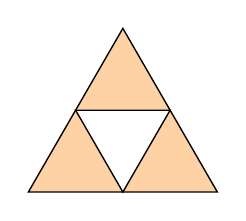
\begin{tikzpicture}[scale=0.8, line width=0.5pt]
  \coordinate (B) at (0,0);
  \coordinate (C) at (3,0);
  \coordinate (A) at (1.5,2.598);
  \coordinate (D) at (0.75,1.299);
  \coordinate (E) at (2.25,1.299);
  \coordinate (F) at (1.5,0);
  \fill[orange!35] (A) -- (D) -- (E) -- cycle;
  \fill[orange!35] (B) -- (F) -- (D) -- cycle;
  \fill[orange!35] (F) -- (C) -- (E) -- cycle;
  \draw (A) -- (B) -- (C) -- cycle;
  \draw (D) -- (E) -- (F) -- cycle;
\end{tikzpicture}
}\end{minipage}\par
\begin{choicesii}{\rule[-3ex]{0pt}{8ex}$\dfrac{243}{4}$}{\rule[-3ex]{0pt}{8ex}$81$}{\rule[-3ex]{0pt}{8ex}$\dfrac{243}{2}$}{\rule[-3ex]{0pt}{8ex}$243$}{\rule[-3ex]{0pt}{8ex}$\dfrac{729}{2}$}\end{choicesii}
